% Adjust these for the path of the theme and its graphics, relative to this file
%\usepackage{beamerthemeFalmouthGamesAcademy}
\usepackage{../../beamerthemeFalmouthGamesAcademy}
\usepackage{multimedia}
\graphicspath{ {../../} }

% Default language for code listings
\lstset{language=C++,
        morekeywords={each,in,nullptr}
}

% For strikethrough effect
\usepackage[normalem]{ulem}
\usepackage{wasysym}

\usepackage{pdfpages}

% http://www.texample.net/tikz/examples/state-machine/
\usetikzlibrary{arrows,automata}

\newcommand{\modulecode}{COMP260}\newcommand{\moduletitle}{Distributed Systems}\newcommand{\sessionnumber}{5}

\begin{document}
\title{\sessionnumber: PS4 Dev Kit \& Profilers}
\subtitle{\modulecode: \moduletitle}

\frame{\titlepage} 

\begin{frame}{Learning outcomes}
	By the end of today's session, you will be able to:
	\begin{itemize}
		\item \textbf{Develop} games for the PS4
		\item \textbf{Understand} the usage of a profiler
		\item \textbf{Profile} your own code base</li>
	\end{itemize}
\end{frame}

\part{Developing for the PS4}
\frame{\partpage}
\part{Coffee Break}
\frame{\partpage}
\part{Profilers}
\frame{\partpage}

\begin{frame}{Unity Profiler}
	\begin{itemize}
		\pause \item The Unity Profiler is built into the engine
		\pause \item It can be accessed via the \textbf{ Window > Profiler}
		\pause \item This allows you to profile the following
		\begin{itemize}
			\pause \item CPU Usage - Scripts, Physics, UI etc
			\pause \item Rendering - Batches, Triangles, Vertices
			\pause \item Memory - Total, Texture, Mesh, Garbage Collection
			\pause \item Audio - Number of Sources, Audio Memory
			\pause \item GPU - Deferred Lighting, Transparent, Post Processing
		\end{itemize} 
	\end{itemize}
\end{frame}

\begin{frame}{Unity Profiler}
	\begin{figure}
		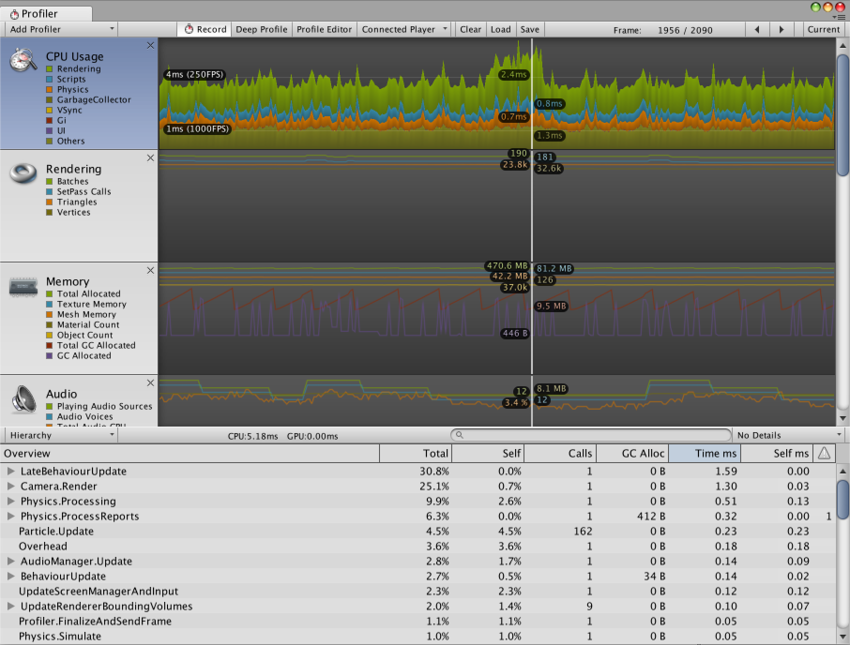
\includegraphics[width=1.0\textwidth,height=0.8\textheight]{UnityProfilerWindow}  
	\end{figure}
\end{frame}

\begin{frame}{Unity Profiler: Hints \& Tips}
	\begin{itemize}
		\pause \item You can remove items from the profiler graph by click on the colour box
		\pause \item Enabling \textbf{Deep Profile} will add a significant overhead to larger games
		\begin{itemize}
			\pause \item Surround you code with \textbf{Profiler.BeginSample} \& \textbf{Profiler.EndSample} this will appear in the Profiler
		\end{itemize}
		\pause \item You should consider Profiling a development build as the Editor adds significant overheard
	\end{itemize}
\end{frame}

\begin{frame}{Unreal Profiler}
	\begin{itemize}
		\pause \item The Unreal Profiler is built into the engine
		\pause \item It can accessed via \textbf{Window > Developer Tools > Session Frontend}
		\pause \item Allows us to profile all major systems
	\end{itemize}
\end{frame}

\begin{frame}{Unreal Profiler}
	\begin{figure}
		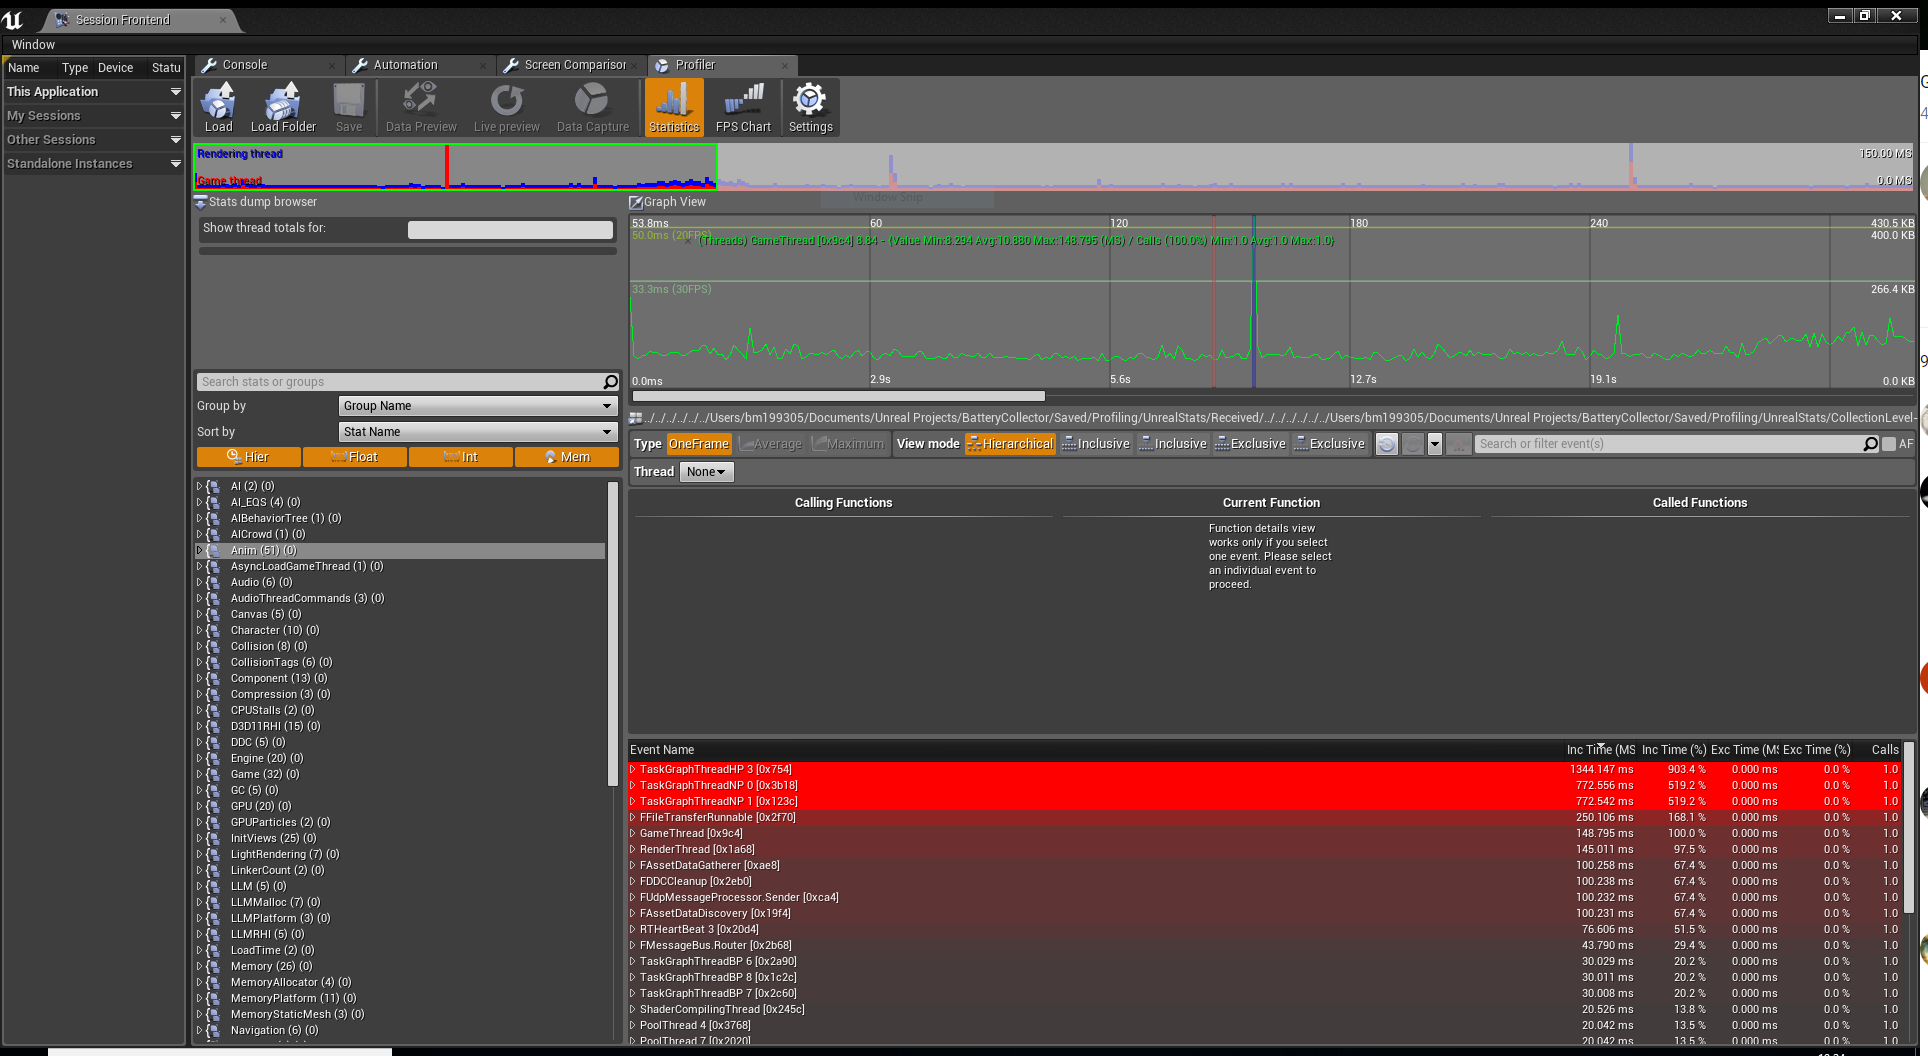
\includegraphics[width=1.0\textwidth,height=0.8\textheight]{UnrealProfilerWindow}  
	\end{figure}
\end{frame}

\end{document}
